%!TEX root = ../report.tex

\section{Design Pattern}

\subsection{Adapter Pattern/Wrapper}
Connects incompatible components to for example
\begin{itemize}
  \item Reuse existing components
  \item Convert an interface to another interface (maybe needed by an API call)
\end{itemize}

Structure:\\
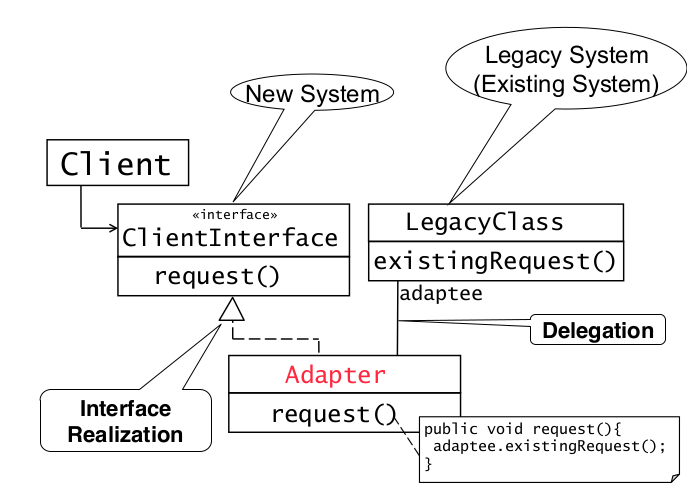
\includegraphics[width=\linewidth]{design_pattern/adapter.png}


\subsection{Bridge Pattern}
Allows to delay the assignment of an implementation of an interface from compile to run time.\\
Structure: \\
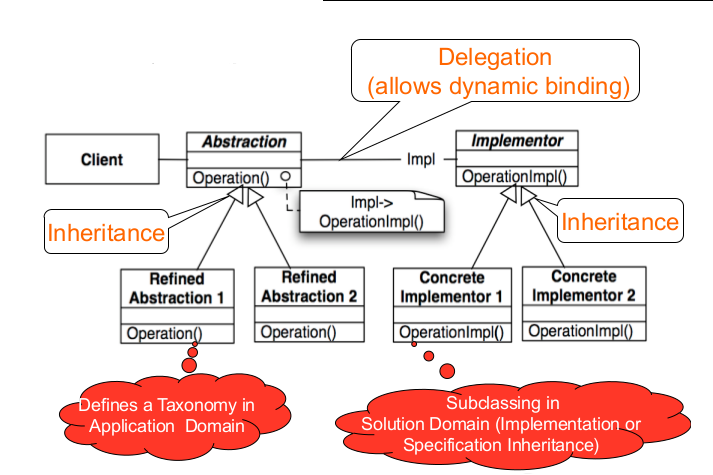
\includegraphics[width=\linewidth]{design_pattern/bridge.png}
The \textbf{degenerated bridge pattern} is the same as the bridge pattern without the taxonomy in the application domain.

\subsection{Proxy Pattern/Caching}
The proxy pattern allows to defer object creation and object initialization to the time you need the object (Remote Proxy (Caching), Substitute (Virtual Proxy), Protection Proxy (Access control/Firewall)).\\
Structure: \\
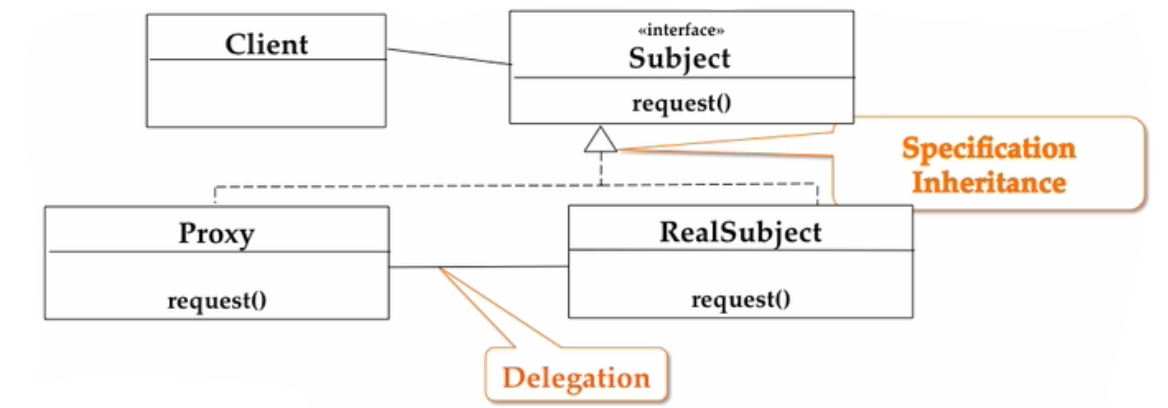
\includegraphics[width=\linewidth]{design_pattern/proxy.png}
The client never calls request() in RealSubject, instead it always calls the method in Proxy which might delegate it to the RealSubject.

\subsection{Composite Pattern}
The composite pattern models tree structures that represent part-whole hierarchies with arbitrary depth and width.
It lets the client treat individual objects and groups uniformly. \\
Structure: \\
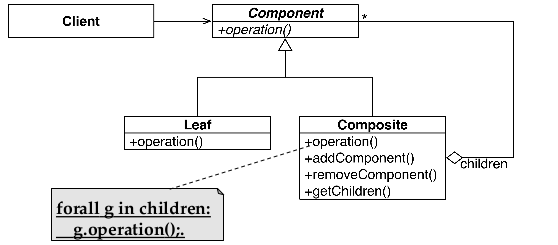
\includegraphics[width=\linewidth]{design_pattern/composite.png}
